\documentclass[12pt]{article}
\usepackage{notes-common}
\usetikzlibrary{calc}
\geometry{margin=0.35in}
\AtBeginDocument{\fontsize{14}{17}\selectfont}

% Complete / filled-in reference version of circuits-devices-notes.tex.
% Mon Oct 12 -- More circuits + devices (Knight 28.5, 28.7).
\newcommand{\ANS}[1]{\textcolor{accent}{#1}}

% ---- same schematic pieces as the skeleton ----
\newcommand{\battv}[1]{% vertical battery symbol centered at (#1)
  \draw[line width=0.7pt] ($(#1)+(0,0.55)$) -- ($(#1)+(0,0.12)$);
  \draw[line width=0.7pt] ($(#1)+(0,-0.12)$) -- ($(#1)+(0,-0.55)$);
  \draw[line width=1.1pt] ($(#1)+(-0.35,0.12)$) -- ($(#1)+(0.35,0.12)$);
  \draw[line width=2.4pt] ($(#1)+(-0.2,-0.12)$) -- ($(#1)+(0.2,-0.12)$);
  \node[scale=0.75] at ($(#1)+(0.6,0.12)$) {$+$};
  \node[scale=0.75] at ($(#1)+(0.6,-0.12)$) {$-$};
}
\newcommand{\reszig}[1]{% horizontal resistor zigzag centered at (#1)
  \fill[white] ($(#1)+(-0.65,-0.32)$) rectangle ($(#1)+(0.65,0.32)$);
  \draw ($(#1)+(-0.6,0)$)
    -- ($(#1)+(-0.42,0.22)$) -- ($(#1)+(-0.24,-0.22)$)
    -- ($(#1)+(-0.06,0.22)$) -- ($(#1)+(0.12,-0.22)$)
    -- ($(#1)+(0.3,0.22)$) -- ($(#1)+(0.48,-0.22)$)
    -- ($(#1)+(0.6,0)$);
}
\newcommand{\metercirc}[2]{% circle labeled #2 at position #1
  \fill[white] ($(#1)+(-0.3,-0.3)$) rectangle ($(#1)+(0.3,0.3)$);
  \draw ($(#1)$) circle (0.3);
  \node[scale=0.8] at (#1) {$#2$};
}
\newcommand{\batthL}[1]{% horizontal battery at (#1), + on the left
  \draw[line width=0.7pt] ($(#1)+(-0.55,0)$) -- ($(#1)+(-0.12,0)$);
  \draw[line width=0.7pt] ($(#1)+(0.12,0)$) -- ($(#1)+(0.55,0)$);
  \draw[line width=1.1pt] ($(#1)+(-0.12,-0.35)$) -- ($(#1)+(-0.12,0.35)$);
  \draw[line width=2.4pt] ($(#1)+(0.12,-0.2)$) -- ($(#1)+(0.12,0.2)$);
  \node[scale=0.75] at ($(#1)+(-0.12,0.55)$) {$+$};
  \node[scale=0.75] at ($(#1)+(0.12,0.55)$) {$-$};
}
\newcommand{\batthR}[1]{% horizontal battery at (#1), + on the right
  \draw[line width=0.7pt] ($(#1)+(-0.55,0)$) -- ($(#1)+(-0.12,0)$);
  \draw[line width=0.7pt] ($(#1)+(0.12,0)$) -- ($(#1)+(0.55,0)$);
  \draw[line width=2.4pt] ($(#1)+(-0.12,-0.2)$) -- ($(#1)+(-0.12,0.2)$);
  \draw[line width=1.1pt] ($(#1)+(0.12,-0.35)$) -- ($(#1)+(0.12,0.35)$);
  \node[scale=0.75] at ($(#1)+(-0.12,0.55)$) {$-$};
  \node[scale=0.75] at ($(#1)+(0.12,0.55)$) {$+$};
}
\newcommand{\reszigv}[1]{% vertical resistor zigzag centered at (#1)
  \fill[white] ($(#1)+(-0.32,-0.65)$) rectangle ($(#1)+(0.32,0.65)$);
  \draw ($(#1)+(0,-0.6)$)
    -- ($(#1)+(0.22,-0.42)$) -- ($(#1)+(-0.22,-0.24)$)
    -- ($(#1)+(0.22,-0.06)$) -- ($(#1)+(-0.22,0.12)$)
    -- ($(#1)+(0.22,0.3)$) -- ($(#1)+(-0.22,0.48)$)
    -- ($(#1)+(0,0.6)$);
}
\newcommand{\twoloopdots}{%
  \filldraw (0,4) circle (1.5pt); \node[scale=0.8, anchor=south east] at (-0.05,4.05) {$e$};
  \filldraw (6,4) circle (1.5pt); \node[scale=0.8, anchor=south west] at (6.05,4.05) {$f$};
  \filldraw (0,2) circle (1.5pt); \node[scale=0.8, anchor=east] at (-0.1,2) {$b$};
  \filldraw (6,2) circle (1.5pt); \node[scale=0.8, anchor=west] at (6.1,2) {$c$};
  \filldraw (0,0) circle (1.5pt); \node[scale=0.8, anchor=north east] at (-0.05,-0.05) {$a$};
  \filldraw (6,0) circle (1.5pt); \node[scale=0.8, anchor=north west] at (6.05,-0.05) {$d$};
}

\begin{document}

\noteshead{More Circuits: Ammeters \& Voltmeters \textcolor{accent}{(completed)}}{}

\goal{
\begin{itemize}[itemsep=5pt,parsep=2pt,topsep=2pt]
\item Meet two measuring devices --- the ammeter and the voltmeter --- and
figure out from first principles what resistance each one must have.
\item See that the loop rule is bigger than ``find the current'': the same
equation lets you solve for \emph{whatever single thing} you don't already
know, once a meter tells you something new.
\item Work three versions of one loop, each with a different unknown.
\end{itemize}}

%============================================================
\nsec{Ideal meters}

\textbf{Ammeter}: measures \ANS{current.} Inserted \ANS{in series} in the
circuit (break the wire, wire the meter into the gap) so the same current
that was already flowing still flows straight through it. An ideal ammeter
has resistance \ANS{$0$.}

\vspace{1mm}
\textbf{Voltmeter}: measures the \ANS{potential difference ($\Delta V$)}
between two points. Connected \ANS{in parallel} across an element (its own
branch, tapping both ends --- it is never spliced into the main wire). An
ideal voltmeter has resistance \ANS{$\infty$ (essentially infinite).}

\checkpoint{An ammeter must not change the current it's reporting; a
voltmeter must not divert any current away from the branch it's tapping.
Given that, which meter needs zero resistance, and which needs (essentially)
infinite resistance?}

{\small\color{accent} The ammeter needs $R=0$: any resistance of its own
would add an extra $IR$ drop and throttle the very current it's trying to
report. The voltmeter needs $R\to\infty$: a finite resistance would give
current an extra path to leak down, siphoning some of it away from the
element being measured. Zero resistance in series, infinite resistance in
parallel --- both add nothing to the loop-rule sum.}

%============================================================
\nsec{Problem 1 --- the current}

A $9.0$ V ideal battery drives current through $R_1=1.8\ \text{k}\Omega$
and $R_2=2.7\ \text{k}\Omega$ in series. An ammeter is wired into the loop
as shown.

\begin{center}
\begin{tikzpicture}[x=1cm,y=1cm]
  \draw (0,0) -- (0,2) -- (7,2) -- (7,0) -- cycle;
  \battv{0,1}
  \node[scale=0.8, anchor=east] at (-0.55,1) {$\varepsilon$};
  \reszig{2,2}
  \node[scale=0.8, anchor=south] at (2,2.45) {$R_1$};
  \reszig{5,2}
  \node[scale=0.8, anchor=south] at (5,2.45) {$R_2$};
  \metercirc{3.5,0}{A}
\end{tikzpicture}
\end{center}

Write the loop rule for this circuit and solve for the current the ammeter
reads.

{\small
Loop rule (the ammeter, $R=0$, contributes no drop of its own):
\[
\varepsilon - IR_1 - IR_2 = 0 \quad\Longrightarrow\quad \varepsilon = I(R_1+R_2).
\]}

\[
\boxed{I = \dfrac{\varepsilon}{R_1+R_2}}
\]

\textbf{Now with the numbers above}:

\[
I = \dfrac{9.0\text{ V}}{1.8\text{ k}\Omega+2.7\text{ k}\Omega}
= \dfrac{9.0\text{ V}}{4.5\text{ k}\Omega} = \ANS{2.0\text{ mA}}
\]

\checkpoint{The ammeter sits on the bottom wire, not between $R_1$ and
$R_2$. Would it read something different if you moved it anywhere else in
this loop? Why?}

{\small\color{accent} No --- this is a single series loop, so the series
rule already says the current is the same everywhere around it. An ideal
ammeter adds no resistance of its own, so sliding it to any other point in
the loop reports that same $2.0$ mA.}

%============================================================
\nsec{Problem 2 --- a voltmeter's reading}

Same loop, but now only $R_1=2.0\ \text{k}\Omega$ and the EMF ($\varepsilon=12$
V) are given --- $R_2$'s resistance is unknown. The ammeter reads
$I=3.0$ mA, and a voltmeter is connected across $R_2$.

\begin{center}
\begin{tikzpicture}[x=1cm,y=1cm]
  \draw (0,0) -- (0,2) -- (7,2) -- (7,0) -- cycle;
  \battv{0,1}
  \node[scale=0.8, anchor=east] at (-0.55,1) {$\varepsilon$};
  \reszig{2,2}
  \node[scale=0.8, anchor=south] at (2,2.45) {$R_1$};
  \reszig{5,2}
  \node[scale=0.8, anchor=south] at (5,2.45) {$R_2$};
  \metercirc{3.5,0}{A}
  \draw[dashed] (4.4,2) -- (4.4,3);
  \draw[dashed] (5.6,2) -- (5.6,3);
  \draw[dashed] (4.4,3) -- (5.6,3);
  \metercirc{5,3}{V}
\end{tikzpicture}
\end{center}

Use the loop rule to predict the voltmeter's reading. (You will not need
$R_2$'s resistance for this part.)

{\small
Loop rule --- the voltmeter's branch carries no current (ideal, $R=\infty$),
so it just reports whatever $\Delta V_2$ the loop rule assigns to that gap:
\[
\varepsilon - IR_1 - \Delta V_2 = 0.
\]}

\[
\boxed{\Delta V_2 = \varepsilon - IR_1}
\]

\textbf{Now with the numbers above}:

\[
\Delta V_2 = 12\text{ V} - (3.0\text{ mA})(2.0\text{ k}\Omega)
= 12\text{ V} - 6.0\text{ V} = \ANS{6.0\text{ V}}
\]

\checkpoint{You found the voltmeter's reading without ever using $R_2$'s
resistance. Why didn't you need it?}

{\small\color{accent} The loop rule only cares about voltage \emph{drops},
not about what causes them. Once you know $\varepsilon$ and the drop across
$R_1$, the remaining drop around the loop is fixed by energy conservation
alone --- whatever resistor (or combination) sits there, it must drop
exactly $6.0$ V to make the loop sum to zero.}

%============================================================
\nsec{Problem 3 --- the EMF itself}

Same loop again, but now the battery's EMF is what's unknown.
$R_1=2.0\ \text{k}\Omega$ is given, the ammeter reads $I=4.0$ mA, and the
voltmeter across $R_2$ reads $5.0$ V.

\begin{center}
\begin{tikzpicture}[x=1cm,y=1cm]
  \draw (0,0) -- (0,2) -- (7,2) -- (7,0) -- cycle;
  \battv{0,1}
  \node[scale=0.8, anchor=east] at (-0.55,1) {$\varepsilon=\,?$};
  \reszig{2,2}
  \node[scale=0.8, anchor=south] at (2,2.45) {$R_1$};
  \reszig{5,2}
  \node[scale=0.8, anchor=south] at (5,2.45) {$R_2$};
  \metercirc{3.5,0}{A}
  \draw[dashed] (4.4,2) -- (4.4,3);
  \draw[dashed] (5.6,2) -- (5.6,3);
  \draw[dashed] (4.4,3) -- (5.6,3);
  \metercirc{5,3}{V}
\end{tikzpicture}
\end{center}

Use the loop rule to find $\varepsilon$.

{\small
Same loop rule, just solved for a different letter this time:
\[
\varepsilon - IR_1 - \Delta V_2 = 0.
\]}

\[
\boxed{\varepsilon = IR_1 + \Delta V_2}
\]

\textbf{Now with the numbers above}:

\[
\varepsilon = (4.0\text{ mA})(2.0\text{ k}\Omega) + 5.0\text{ V}
= 8.0\text{ V} + 5.0\text{ V} = \ANS{13.0\text{ V}}
\]

\checkpoint{Using $I$ and the voltmeter reading, could you now find $R_2$
too, even though its resistance was never given directly? What is it?}

{\small\color{accent} Yes --- Ohm's law on $R_2$ alone: $R_2=\Delta
V_2/I=5.0\text{ V}/4.0\text{ mA}=\ANS{1.25\text{ k}\Omega}$. Across all
three problems, the loop rule plus one meter reading was always enough to
pin down whichever single quantity was missing.}

%============================================================
\nsec{Two loops, two batteries}

A single loop only ever gives you \emph{one} equation. The circuit below
has three branches meeting at $b$ and at $c$, so there are three unknown
currents $I_1,I_2,I_3$ --- one loop equation can't pin down three unknowns.

\textbf{How many equations do you need, and where does each one come
from?} \ANS{Three: pick any \emph{two} of the loop's windows (a third loop
is just their sum, not new information) and add the junction rule at $b$
or $c$.}

\checkpoint{Why doesn't the loop rule applied to the \emph{outer} perimeter
($e$-$f$-$d$-$a$-$e$) give you a fourth, independent equation?}

{\small\color{accent} Walking the outer perimeter is the same as walking
Loop 1 and Loop 2 back to back --- the shared $b$-$c$ branch gets traversed
once each way, so its terms cancel and you're left with exactly Loop 1 +
Loop 2 added together. It's a true statement, just not an \emph{independent}
one.}

%============================================================
\nsec{Problem 4 --- all three currents}

In the circuit below, $\varepsilon_1=9.0$ V, $R_1=4\ \Omega$,
$\varepsilon_2=16$ V, $R_2=5\ \Omega$, $R_3=2\ \Omega$.

\begin{center}
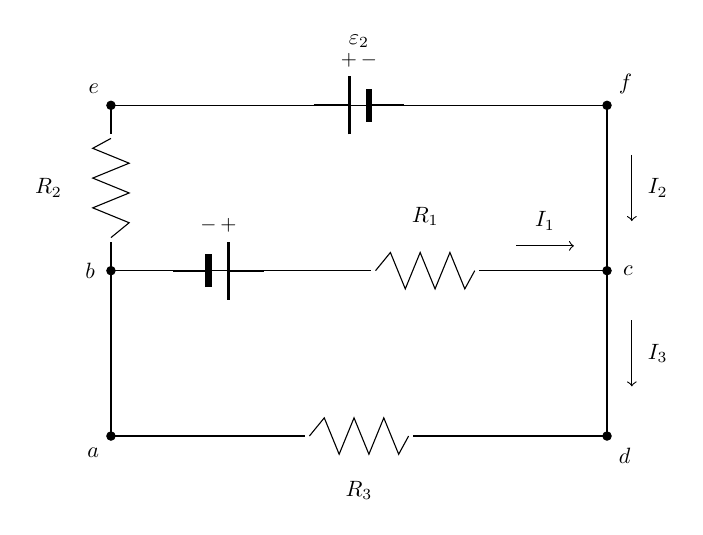
\begin{tikzpicture}[x=1.05cm,y=1.05cm]
  \draw (0,0) -- (0,4) (6,0) -- (6,4) (0,4) -- (6,4) (0,0) -- (6,0) (0,2) -- (6,2);
  \batthL{3,4}
  \node[scale=0.8, anchor=south] at (3,4.6) {$\varepsilon_2$};
  \reszigv{0,3}
  \node[scale=0.8, anchor=east] at (-0.5,3) {$R_2$};
  \batthR{1.3,2}
  \reszig{3.8,2}
  \node[scale=0.8, anchor=south] at (3.8,2.45) {$R_1$};
  \draw[->] (4.9,2.3) -- (5.6,2.3);
  \node[scale=0.8] at (5.25,2.6) {$I_1$};
  \draw[->] (6.3,3.4) -- (6.3,2.6);
  \node[scale=0.8, anchor=west] at (6.4,3) {$I_2$};
  \draw[->] (6.3,1.4) -- (6.3,0.6);
  \node[scale=0.8, anchor=west] at (6.4,1) {$I_3$};
  \reszig{3,0}
  \node[scale=0.8, anchor=north] at (3,-0.45) {$R_3$};
  \twoloopdots
\end{tikzpicture}
\end{center}

Write the loop rule for each loop and the junction rule at $c$, then solve
the resulting system for all three currents.

{\small
\[
I_1R_1-I_2R_2=\varepsilon_1+\varepsilon_2 \quad\Rightarrow\quad 4I_1-5I_2=25
\]
\[
I_1R_1+I_3R_3=\varepsilon_1 \quad\Rightarrow\quad 4I_1+2I_3=9
\]
\[
I_1+I_2=I_3
\]
Substituting $I_3=I_1+I_2$ into the second equation gives
$4I_1+2(I_1+I_2)=9 \Rightarrow 6I_1+2I_2=9$. Combined with
$4I_1-5I_2=25$, eliminate $I_2$: multiply the first by $2$ and the second
by $5$, then add:}

\[
I_1 = \ANS{2.5\text{ A}} \qquad I_2 = \ANS{-3.0\text{ A}} \qquad
I_3 = I_1+I_2 = \ANS{-0.5\text{ A}}
\]

\checkpoint{One of your currents came out negative. What does that tell you
about the direction you assumed for it on the diagram?}

{\small\color{accent} Both $I_2$ and $I_3$ came out negative --- the actual
current in each of those branches flows opposite to the arrow drawn. $I_1$
came out positive, so that arrow was right. Check: $I_1R_1-I_2R_2=
2.5(4)-(-3.0)(5)=10+15=25=\varepsilon_1+\varepsilon_2$, and
$I_1R_1+I_3R_3=2.5(4)+(-0.5)(2)=10-1=9=\varepsilon_1$. \checkmark}

%============================================================
\nsec{Problem 5 --- an unknown resistor}

Same shape, new numbers: $\varepsilon_1=20$ V, $R_1=3\ \Omega$,
$\varepsilon_2=10$ V, $R_2=5\ \Omega$. This time $R_3$ is unknown --- but an
ammeter in the $\varepsilon_1$-$R_1$ branch reads $I_1=4.0$ A.

\begin{center}
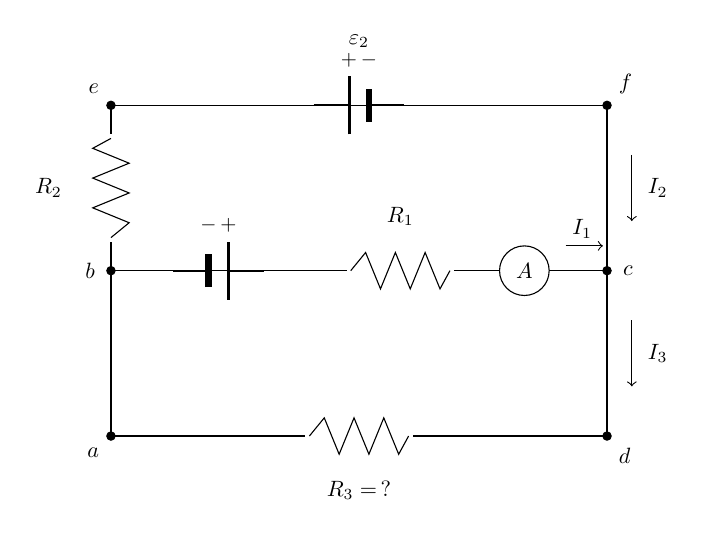
\begin{tikzpicture}[x=1.05cm,y=1.05cm]
  \draw (0,0) -- (0,4) (6,0) -- (6,4) (0,4) -- (6,4) (0,0) -- (6,0) (0,2) -- (6,2);
  \batthL{3,4}
  \node[scale=0.8, anchor=south] at (3,4.6) {$\varepsilon_2$};
  \reszigv{0,3}
  \node[scale=0.8, anchor=east] at (-0.5,3) {$R_2$};
  \batthR{1.3,2}
  \reszig{3.5,2}
  \node[scale=0.8, anchor=south] at (3.5,2.45) {$R_1$};
  \metercirc{5,2}{A}
  \draw[->] (5.5,2.3) -- (5.95,2.3);
  \node[scale=0.8, anchor=south] at (5.7,2.3) {$I_1$};
  \draw[->] (6.3,3.4) -- (6.3,2.6);
  \node[scale=0.8, anchor=west] at (6.4,3) {$I_2$};
  \draw[->] (6.3,1.4) -- (6.3,0.6);
  \node[scale=0.8, anchor=west] at (6.4,1) {$I_3$};
  \reszig{3,0}
  \node[scale=0.8, anchor=north] at (3,-0.45) {$R_3=\,?$};
  \twoloopdots
\end{tikzpicture}
\end{center}

Use the loop rule and the junction rule to find $R_3$. (Work out $I_2$,
then $I_3$, on your way there.)

{\small
Loop 1 is the only equation with $\varepsilon_2$ and $R_2$ in it, and $I_1$
is now known, so solve it for $I_2$ first:
\[
I_1R_1-I_2R_2=\varepsilon_1+\varepsilon_2 \;\Rightarrow\;
3(4)-5I_2=20+10 \;\Rightarrow\; I_2=\ANS{-3.6\text{ A}}
\]
Junction rule:
\[
I_3=I_1+I_2=4.0+(-3.6)=\ANS{0.4\text{ A}}
\]
Loop 2 is the only equation with $R_3$ in it:
\[
\varepsilon_1=I_1R_1+I_3R_3 \;\Rightarrow\; 20=3(4)+0.4R_3
\]}

\[
\boxed{R_3 = \dfrac{\varepsilon_1-I_1R_1}{I_3}} \qquad
R_3=\dfrac{20-12}{0.4}=\ANS{20\ \Omega}
\]

\checkpoint{Could you have found $R_3$ without first finding $I_2$? Why or
why not?}

{\small\color{accent} No. $R_3$ only shows up in Loop 2, and Loop 2 has two
unknowns in it, $I_3$ and $R_3$, until $I_3$ is pinned down. $I_3$ only
comes from the junction rule, which needs $I_2$ --- and $I_2$ only comes
from Loop 1 (the one equation that actually contains $\varepsilon_2$ and
$R_2$). Every given number gets used along exactly one chain.}

%============================================================
\nsec{Problem 6 --- an unknown EMF}

Same shape again: $R_1=5\ \Omega$, $R_2=6\ \Omega$, $R_3=4\ \Omega$. This
time $\varepsilon_2$ is unknown, but $\varepsilon_1=21$ V is given, and the
ammeter reads $I_1=3.0$ A.

\begin{center}
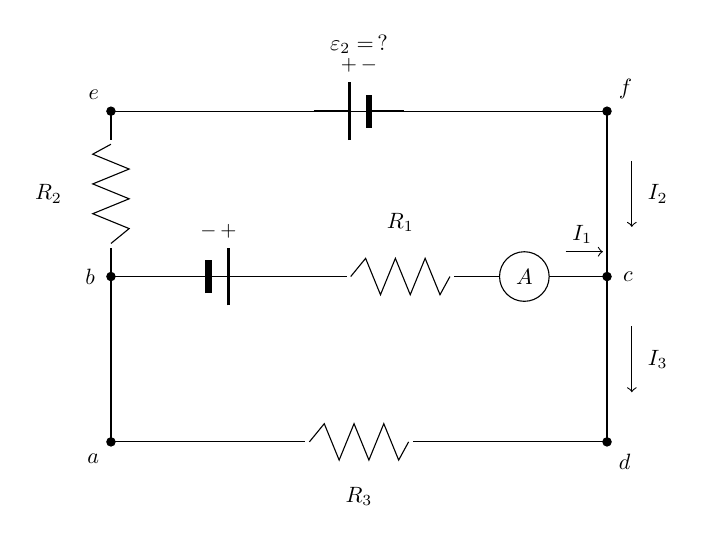
\begin{tikzpicture}[x=1.05cm,y=1.05cm]
  \draw (0,0) -- (0,4) (6,0) -- (6,4) (0,4) -- (6,4) (0,0) -- (6,0) (0,2) -- (6,2);
  \batthL{3,4}
  \node[scale=0.8, anchor=south] at (3,4.6) {$\varepsilon_2=\,?$};
  \reszigv{0,3}
  \node[scale=0.8, anchor=east] at (-0.5,3) {$R_2$};
  \batthR{1.3,2}
  \reszig{3.5,2}
  \node[scale=0.8, anchor=south] at (3.5,2.45) {$R_1$};
  \metercirc{5,2}{A}
  \draw[->] (5.5,2.3) -- (5.95,2.3);
  \node[scale=0.8, anchor=south] at (5.7,2.3) {$I_1$};
  \draw[->] (6.3,3.4) -- (6.3,2.6);
  \node[scale=0.8, anchor=west] at (6.4,3) {$I_2$};
  \draw[->] (6.3,1.4) -- (6.3,0.6);
  \node[scale=0.8, anchor=west] at (6.4,1) {$I_3$};
  \reszig{3,0}
  \node[scale=0.8, anchor=north] at (3,-0.45) {$R_3$};
  \twoloopdots
\end{tikzpicture}
\end{center}

Find $\varepsilon_2$. (This time work out $I_3$ first, then $I_2$.)

{\small
Loop 2 is the only equation with $R_3$ in it, and it only involves $I_1$
and $I_3$ --- solve it first:
\[
\varepsilon_1=I_1R_1+I_3R_3 \;\Rightarrow\; 21=3(5)+4I_3 \;\Rightarrow\;
I_3=\ANS{1.5\text{ A}}
\]
Junction rule:
\[
I_2=I_3-I_1=1.5-3.0=\ANS{-1.5\text{ A}}
\]
Loop 1 is the only equation with $\varepsilon_2$ in it:
\[
I_1R_1-I_2R_2=\varepsilon_1+\varepsilon_2 \;\Rightarrow\;
3(5)-(-1.5)(6)=21+\varepsilon_2
\]}

\[
\boxed{\varepsilon_2 = I_1R_1-I_2R_2-\varepsilon_1} \qquad
\varepsilon_2 = 15+9-21=\ANS{3.0\text{ V}}
\]

\checkpoint{Compare the order you worked in for Problems 5 and 6 --- which
loop did you need \emph{first} in each, and why did the unknown force that
order?}

{\small\color{accent} Problem 5's unknown ($R_3$) lives only in Loop 2, but
Loop 2 was stuck with two unknowns ($I_3$ and $R_3$) until $I_2$ --- found
from Loop 1 --- fed the junction rule. Problem 6's unknown ($\varepsilon_2$)
lives only in Loop 1, but Loop 1 needed $I_2$, which needed $I_3$ from Loop
2 first. Whichever loop \emph{doesn't} contain the unknown is always the
one you solve first --- it's the one that's already fully determined by
what you're given.}

\end{document}
